\documentclass[12pt,a4paper]{article}

\usepackage{microtype}% si on encode direct en pdf
\usepackage[utf8]{inputenc}% pour compatibilité maximale
\usepackage[T1]{fontenc}% pour le français
%\usepackage{lmodern}
\usepackage[light, oldstylenums, nott,%
    narrowiints, uprightgreeks, partialup]{kpfonts}
\usepackage[scaled]{beramono}% belle mécane avec bold
\usepackage[french]{babel}%  pour le français

\usepackage[noload=abbr]{siunitx}% sans les abbréviations
\sisetup{decimalsymbol=comma}% pour la virgule.
\sisetup{expproduct=tighttimes}% pour l'écriture scientifique ressérée.
\sisetup{trapambigfrac,openfrac=(,closefrac=),per=slash}
% pour pas effrayer nos petits collégiens, et en restant prudent.
%
%\renewunit{\litre}{l }    % C'est le choix par défaut. L c'est \liter par défaut.
%\renewunit{\litre}{L }    %Pour la version officielle
\renewunit{\litre}{\ell } % je trouve que c'est mieux pour les litres
%c'est bien sûr discutable, ce n'est pas officellement le choix du SI


\usepackage{pifont}%Pour les symboles ding
\usepackage{marvosym}% pour plein de symboles, attention avec eurosym !!!
\usepackage{eurosym}% pour le symbole euro, mieux que marvosym.
\let\EURbis\EUR
\renewcommand\EUR[1]{\text{\EURbis{\num{#1}}}}
%utilisation ex: \EUR{35.4} (ou \EUR{35,4}) en mode texte (ou math), ou \euro\ tout seul.
%
%
%
\usepackage{enumerate}% pour choisir le style dans la numérotation. TB
%
%
\usepackage{fancybox}% pour de jolies boites \ovalvox{texte} ou \shadowbox{texte}
\usepackage{multicol}% pour multicolones
\usepackage{frcursive}% pour écrire comme à l'école
%\usepackage{cancel}% pour simplifier les fractions
%
\usepackage{fancyhdr}%pour personnaliser les en-têtes et pieds de page
%
%
%
\usepackage{graphicx}% insertion de graphique
%
% pour un joli (AB)//(CD)
%\renewcommand{\parallel}{\mathrel{/\!/}}% avec de l'espace.
\renewcommand{\parallel}{\mathclose{}/\!/\mathopen{}}% plus resséré
%\renewcommand{\parallel}{/\!/}% Too Bad

\usepackage{pstricks,pst-plot,pst-tree,pstricks-add}


\usepackage{geometry}
\geometry{lmargin=2.5cm,rmargin=0cm,vmargin={0.5cm,0.5cm},twoside,includeall}

\setlength\parindent{0mm}
%
\usepackage{xcolor}%pour de la couleur
\definecolor{cPG}{RGB}{235, 227, 150}
\definecolor{link}{RGB}{150, 81, 0}
\usepackage[colorlinks, linkcolor=link]{hyperref}

%%%%%%%COULEURS%%%%%%
\definecolor{my-gray}{gray}{0.95}
\colorlet{fond-code}{my-gray}
\colorlet{bord-code}{cyan}
\colorlet{comment}{link}
\colorlet{c-emph}{blue}
\colorlet{c-key}{red}
\colorlet{c-math}{olive}


\usepackage{listings}
\lstset{extendedchars=true,
literate={é}{{\'e}}1 {è}{{\`e}}1 {à}{{\`a}}1 {ç}{{\c{c}}}1 {œ}{{\oe}}1 {ù}{{\`u}}1
{É}{{\'E}}1 {È}{{\`E}}1 {À}{{\`A}}1 {Ç}{{\c{C}}}1 {Œ}{{\OE}}1 {Ê}{{\^E}}1
{ê}{{\^e}}1 {î}{{\^i}}1 {ô}{{\^o}}1 {û}{{\^u}}1
{§}{{\S}}1 {°}{{\textdegree}}1 {±}{{\textpm}}1 {'}{{\textquotesingle}}1
 }


\lstset{%
language=python,
keywords=[1]{and,as,assert,break,class,continue,def,%
del,elif,else,except,False,finally,for,%
from,global,if,import,in,is,lambda,%
None,nonlocal,not,or,pass,raise,return,%
True,try,while,with,yield},
%
keywords=[2]{print,input,str,float,int,len,range,abs,%
any,all,set,sum,pow,sorted,list,divmod,enumerate,ord,open,min,max,dir},
keywordstyle=[1]\bfseries\color{red},
keywordstyle=[2]\color{brown},
numbers=none,
escapechar=§,
string=[b]",
%morestring=[b]\textquotesingle,
stringstyle=\color{purple},
moredelim=[is][\ttfamily\color{blue}]{£}{£},
moredelim=[is][\ttfamily\color{red}]{≤}{≥}%erreur de python, en rouge
}
\renewcommand*{\lstlistlistingname}{Codes sources des programmes \sujet}
\renewcommand*{\lstlistingname}{Code source}

\lstset{%
basicstyle=\ttfamily,  
       % the size of the fonts that are used for the code
numbers=left, 
               % where to put the line-numbers
numberstyle=\footnotesize,
  % the size of the fonts that are used for the line-numbers
stepnumber=1,  
   % the step between two line-numbers. If it's 1 each line 
                                % will be numbered
numbersep=5pt, 
                 % how far the line-numbers are from the code
backgroundcolor=\color{fond-code}, 
      % choose the background color. You must add \usepackage{color}
showspaces=false, 
               % show spaces adding particular underscores
showstringspaces=false, 
        % underline spaces within strings
showtabs=false,   
              % show tabs within strings adding particular underscores
frame=single,	  
              % adds a frame around the code
tabsize=4,	  
              % sets default tabsize to 4 spaces
captionpos=b,   
              % sets the caption-position to bottom
breaklines=true, 
               % sets automatic line breaking
breakatwhitespace=false,    
    % sets if automatic breaks should only happen at whitespace
title=\lstname,    
             % show the filename of files included with \lstinputlisting;
                                % also try caption instead of title
escapeinside={*!}{!*},    
     % if you want to add a comment within your code
%morekeywords={???}            % if you want to add more keywords to the set
framexleftmargin=5mm, frame=shadowbox, rulesepcolor=\color{bord-code},
commentstyle=\color{comment}\small,
emphstyle=\color{c-emph},
keywordstyle=\ttfamily\bfseries\color{c-key},
}% à compléter au besoin
%
%

\begin{document}
\thispagestyle{empty}

\ovalbox{CERI --- Licence --- INFO --- Semestre 2 --- Mathématiques discrètes --- 3 mai 2018}

\bigskip

\begin{center}

   {\Large \textbf{Évaluation écrite -- Arithmétique}}
   
   \medskip

   {\Large \textbf{Durée 1h20}}
   
   \medskip
   
   \emph{Seule la calculatrice de type collège \textbf{(non programmable)} est autorisée.}
   
   
   \medskip
   
   \emph{Il est inutile de finir tout le sujet pour avoir la note maximale.}
   
  

\end{center}


\vspace*{\stretch{1}}

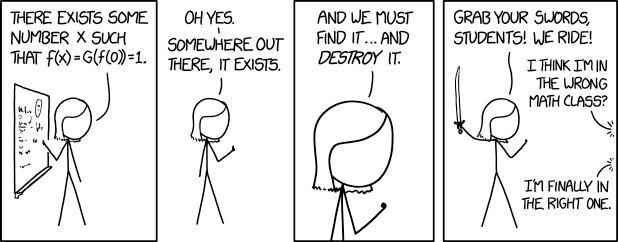
\includegraphics[scale=0.7]{exi}

\texttt{https://xkcd.com/1856/}

\vspace*{\stretch{1}}

\pagebreak





  Dans tout le devoir, vous pourrez utiliser sans preuve que :
\begin{itemize}
\item   $257$ et \num{1000000009} sont des nombres premiers.

\end{itemize}  
 

%==============================================================
\section*{I] Je sais calculer un PGCD ($10$ points)}
\begin{enumerate}
\item Donner la décomposition en facteurs premiers de $A = 1326$ et $B = 75000000675$. \emph{Inutile de justifier ici.}
\item Calculer $\textrm{PGCD}(1326, 1482)$ avec deux méthodes différentes. \emph{On attend le nom des méthodes et une présentation correcte des calculs, ainsi qu'une phrase de conclusion.}
\item Calculer $\textrm{PGCD}(\num{98882}, \num{99862})$. \emph{Donner quelques détails de calculs, le résultat seul ne rapporte aucun point.}
\item Calculer $\textrm{PGCD}(\num{1000000009}, \num{2000000018})$. \emph{Donner quelques détails sur votre méthode.}
\end{enumerate}


\section*{II] Je sais trouver la liste des diviseurs ($7$ points)}
\begin{enumerate}
\item Donner la liste des diviseurs de $930$. \emph{On attend une bonne présentation des calculs.}
\item On a demandé à Alice et à Bob de faire un script qui donne la somme des diviseurs d'un entier naturel non nul.

Ces scripts sont faux, trouver la ou les erreurs. Les erreurs sont de petits oublis ou des caractères échangés. \emph{On n'attend pas une réécriture, ni votre version. On attend que les petites erreurs soient identifiées et corrigées.}
\end{enumerate}

\lstset{frameround=fttt}

\begin{lstlisting}[language=Python, frame=trBL]
def somDiv(n):
    "Somme des diviseurs de n, par Alice"
    S = 0
    for x in range(1, n):
        if x*x>n: break
        if n%x == 0:
           S += x + x//n
           if x*x == n:
               S -= x
    return S
\end{lstlisting}

\begin{lstlisting}[language=Python, frame=trBL]
def somDiv(n):
    "Somme des diviseurs de n, par Bob"
    S = 0
    for x in range(1, n+1):
        if x%n == 0:
           S += n
    return S
\end{lstlisting}


\section*{II] Je sais déterminer si un nombre est premier ($8$ points)}
\begin{enumerate}
\item Pour chacun des nombres suivants, dire s'il est composé ou premier.
 \emph{Justifier le.}
 
 $$n_1 = 221,\; n_2=139,\; n_3=\num{90000000000000300000000081}, \;n_4 = \num{102509874063005}$$

\item Xerk possède la liste des nombres premiers jusqu'à $65537$, et il assure qu'aucun d'eux ne divise ni $n_5$, ni $n_6$. \emph{On peut le croire !}

Les nombre $n_5 = \num{4296409193}$ et $n_6=4295098349$ sont-ils premiers ou non ? \emph{Justifier.}

\item Les nombres premiers jumeaux sont des nombres premiers de la forme $(p, p+2)$, comme par exemple : $(5, 7)$, ou bien $(11, 13)$. Est-il possible d'avoir des nombres premiers triplets, de la forme $(p, p+2, p+4)$ ? \emph{Justifier.}

\item Donner le nom d'une méthode qui détermine tous les nombres premiers dans un intervalle.
\end{enumerate}

\section*{III] VRAI ou FAUX ? ($11$ points)}
Pour cet exercice, il est inutile de justifier. Présenter ses réponses sur deux colonnes bien alignées : une avec le numéro de la question, l'autre avec VRAI ou FAUX.
\begin{enumerate}
\item $9197 = 17\times540 + 17$.
\item $9197$ modulo $540$ est égal à $17$.
\item $9197$ modulo $17$ est égal à $17$.
\item Avec $a$, $b$, $c$, $u$, $v\in \mathbb{Z}$, si $a\mid b$ et $a\mid c$, alors $a\mid ub+vc$.
\item Pour $a\in \mathbb{Z}$, on $a\land 1 = 1$, même pour $a=0$.
\item Pour $k\in \mathbb{Z}$, on a $7(3k+1) - 3(7k+2)=1$.
\item Pour $k\in \mathbb{Z}$, on a $(3k+1) \land (7k+2)=1$.
\item Pour $k\in \mathbb{Z}$, $3$ est un inverse de $7k+2$, modulo $3k+1$.
\item Pour $k\in \mathbb{Z}$, $7$ est un inverse de $3k+1$, modulo $7k+2$.
\item $2^7\times 7^2$ est la décomposition en facteurs premiers de $6872$.
\item $2^7\times 51$ est la décomposition en facteurs premiers de $6528$.
\end{enumerate}

\section*{IV] Je sais utiliser une formule ($6$ points)}
On rappelle que les fonctions nombre de diviseurs, somme des diviseurs, et indicatrice d'Euler sont des fonctions arithmétiques multiplicatives. Elles vérifient donc en tant que $f$ :
 $$\forall u, v \in \mathbb{N}^*, u\land v = 1 \implies f(uv) = f(u)f(v)$$

On rappelle de plus, pour $p$ un nombre premier, et $e\in\mathbb{N}^*$ , que :
\begin{itemize}
\item Le nombre de diviseurs de $p^e$ est $e+1$.
\item La somme des diviseurs de $p^e$ est $\dfrac{p^{e+1}-1}{p-1}$.
\item L'indicatrice d'Euler de $p^e$ est $p^{e-1}(p-1)$.

\begin{enumerate}
\item Vérifier que $\num{362880} = 2^e\times 3^4 \times 5 \times 7$, où $e$ est un entier à déterminer.
\item Vérifier que le nombre de diviseurs de $\num{362880}$ est égal à $160$.
\item Calculer la somme des diviseurs de $\num{362880}$.
\item Calculer l'indicatrice d'Euler de $\num{362880}$.

\end{enumerate}

\end{itemize}

\section*{V] Je fais de l'arithmétique modulaire simple ($5$ points)}
\emph{Toutes les réponses doivent être justifiées.}
\begin{enumerate}
\item Montrer que $3^2 \equiv -1 \pmod {10}$.
\item En déduire que $3^4 \equiv 1 \pmod {10}$.
\item Montrer que $403 \equiv 3 \pmod {4}$.
\item Quel est le dernier chiffre de $3^{403}$ ?
\item Quel est le dernier chiffre de $3^{(403^{42})}$ ?
\end{enumerate}

\section*{VI] Je sais évaluer un polynôme ($5$ points)}
On considère le polynôme $P(x) = 3x^5 -2x^4 +5x^2 +x -1$, on ne s'intéresse qu'aux résultats modulo $257$.
\begin{enumerate}
\item Vérifier que $P(0)$ mod $257 = 256$.
\item Calculer $P(1)$ mod $257$.
\item Calculer $P(111)$ mod $257$.
\end{enumerate}

\section*{VII] Je sais résoudre des équations simples ($5$ points)}
\begin{enumerate}
\item Résoudre l'équation où $x\in\mathbb{Z}$ :
$$6x\equiv 12 \pmod{27}$$
\item Résoudre le système où $x, y\in\mathbb{Z}$ :
\end{enumerate}
    $$\left\{
    \begin{array}{r c l}
       x +2y & \equiv &6 \pmod{7} \\
       5x +4y & \equiv &3 \pmod{7} \\
    \end{array}
    \right.$$

\section*{VIII] Je sais calculer un inverse modulaire ($3$ points)}
Montrer que $31$ est inversible modulo $100$, et proposer un inverse.

\vspace*{\stretch{1}}
\thispagestyle{empty}

\begin{center}
  \begin{cursive}Fin du sujet\end{cursive} 
\end{center}

\end{document}